\documentclass[tikz,border=2pt]{standalone}
\usepackage{amsmath}
\usepackage{pgfplots}
\pgfplotsset{compat=1.18}
\usetikzlibrary{arrows.meta}
\begin{document}
% Example 4.6: V={x1<=4, -2x1+x2<=6, -x1-x2<=-3, x1-x2<=1}, extreme points (4,3),(4,14),(-1,4),(2,1);
% f=12-x1-x2 has level lines x1+x2=const: f=9 contains the edge [(-1,4),(2,1)] (maximizers), f=5 through (4,3), min f=-6 at (4,14).
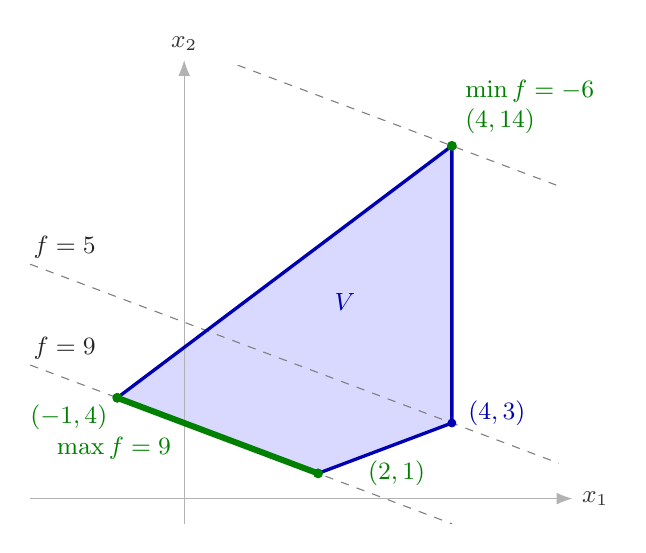
\begin{tikzpicture}[font=\small, >={Latex[length=2mm]}, x=0.85cm, y=0.32cm]
  \begin{scope}
    \clip (-2.3,-1) rectangle (5.6,17.2);
    \fill[blue!15] (2,1) -- (4,3) -- (4,14) -- (-1,4) -- cycle;
    % level lines of f
    \draw[gray, dashed] (-2.3,5.3) -- (4,-1);
    \draw[gray, dashed] (-2.3,9.3) -- (5.6,1.4);
    \draw[gray, dashed] (0.8,17.2) -- (5.6,12.4);
  \end{scope}
  \draw[gray!60, ->] (-2.3,0) -- (5.8,0) node[anchor=west, gray!40!black] {$x_1$};
  \draw[gray!60, ->] (0,-1) -- (0,17.4) node[anchor=south, gray!40!black] {$x_2$};
  \draw[blue!70!black, very thick] (2,1) -- (4,3) -- (4,14) -- (-1,4);
  % maximizers: the whole edge on x1+x2=3
  \draw[green!50!black, line width=2.2pt] (-1,4) -- (2,1);
  \foreach \p in {(-1,4),(2,1),(4,14)} \fill[green!50!black] \p circle (1.8pt);
  \fill[blue!70!black] (4,3) circle (1.6pt);
  % labels
  \node[gray!30!black, anchor=south west, inner sep=1pt] at (-2.3,9.4) {$f=5$};
  \node[gray!30!black, anchor=south west, inner sep=1pt] at (-2.3,5.4) {$f=9$};
  \node[green!50!black, anchor=south west, align=left, inner sep=1pt] at (4.15,14.35) {$\min f=-6$\\$(4,14)$};
  \node[green!50!black, anchor=north east, inner sep=1pt] at (-1.1,3.85) {$(-1,4)$};
  \node[green!50!black, anchor=west, inner sep=1pt] at (2.7,1.0) {$(2,1)$};
  \node[green!50!black, anchor=north east, inner sep=1pt] at (-0.15,2.55) {$\max f=9$};
  \node[blue!70!black, anchor=west] at (4.1,3.4) {$(4,3)$};
  \node[blue!70!black] at (2.4,7.8) {$V$};
\end{tikzpicture}
\end{document}
